\chapter{HASIL DAN ANALISIS}
\label{chap:pengujiananalisis}

% Ubah bagian-bagian berikut dengan isi dari pengujian dan analisis

Pada penelitian ini dipaparkan mengenai pengujian dari model yang dibuat pada metodologi sebelumnya. Hasil pengujian kemudian akan dianalisis dan diharapkan dari hasil analisis didapatkan kesimpulan mengenai model yang dibuat dengan metode yang telah ditentukan.

\section{Hasil Pengumpulan Dataset}
\label{sec:HasilPengumpulanDataset}
Dengan Menggunakan dataset yang dimiliki dengan total video sebanyak 36 video untuk dataset DROZY dan 36 video untuk dataset UTA-RLDD. Kemudian berdasarkan nilai KSS yang dimiliki tiap dataset, video dikelompokkan berdasarkan kelas yang telah ditentukan. Pada penelitian ini digunakan 3 kelas klasifikasi yaitu Fokus sebagai kelas 1, kemudian waspada sebagai kelas 2, dan mengantuk sebagai kelas 3. Setelah dilakukan pengelompokan maka didapatkan jumlah video tiap kelas nya sebanyak 72 video seperti pada tabel berikut :

\begin{longtable}{|c|c|}
  \caption{Hasil Pengumpulan Video Dataset DROZY}
  \label{tb:HasilDrozy}                                   \\
  \hline
  \rowcolor[HTML]{C0C0C0}
  \textbf{Kelas} & \textbf{Total Video} \\
  \hline
  1            & 11  \\              
  2            & 10  \\              
  3            & 15  \\                           
  \hline
\end{longtable}


\begin{longtable}{|c|c|}
  \caption{Hasil Pengumpulan Video Dataset UTA-RLDD}
  \label{tb:HasilUTA}                                   \\
  \hline
  \rowcolor[HTML]{C0C0C0}
  \textbf{Kelas} & \textbf{Total Video} \\
  \hline
  1            & 12  \\              
  2            & 12  \\              
  3            & 12  \\                           
  \hline
\end{longtable}

\section{Hasil Ekstraksi Openness dan MAR}
\label{sec:skenariopengujian}
Kemudian dengan menggunakan video yang telah disaring sebagai dataset, maka dilakukan ekstraksi nilai PERCLOS dan MAR secara bersamaan. Pada penelitian ini digunakan DLib sebagai library untuk mengekstrak fitur mata dan mulut untuk kemudian dicari nilai PERCLOS dan MAR nya. Untuk MAR sendiri, prinsip yang digunakan untuk mendapatkan nilai MAR nya adalah sama dengan menggunakan rumus yang ada pada rumus 2.2. Sedangkan untuk mendapatkan nilai perclos, digunakan metode grayscaling untuk mengubah bagian mata menjadi hitam dan putih dimana selanjutnya bagian tersebut diubah menjadi nilai binary yang kemudian digunakan untuk menghitung nilai PERCLOS. Sehingga pada saat video dataset digunakan dan diekstraksi, didapatkan hasil seperti pada tabel berikut :

\begin{longtable}{|c|c|c|}
  \caption{Hasil Ekstraksi Openness dan MAR}
  \label{tb:openessMar}                                   \\
  \hline
  \rowcolor[HTML]{C0C0C0}
  \textbf{Frame} & \textbf{Openness} & \textbf{MAR\_Std} \\
  \hline
  1     & 0.33275762637414663 & 0.38539513718352214 \\
2     & 0.34874697414643113 & 0.4205568267370099  \\
3     & 0.360703620018165   & 0.40674460840998033 \\
4     & 0.3507866493276178  & 0.4029997011463999  \\
5     & 0.37454249196259926 & 0.4044786041022079  \\
6     & 0.3634563454911023  & 0.4044786041022079  \\
7     & 0.3321819194149599  & 0.3992242079377172  \\
8     & 0.3504649829636901  & 0.3992242079377172  \\
9     & 0.35549913081642326 & 0.4205568267370099  \\
10    & 0.3321819194149599  & 0.38539513718352214 \\
11    & 0.39724856953743126 & 0.441461136857296   \\
12    & 0.396521810060564   & 0.4817688377401808  \\
13    & 0.37037209526233333 & 0.42857142857142855 \\
14    & 0.39879948581769054 & 0.43103448275862066 \\
15    & 0.3049122660070178  & 0.5163798686058965  \\
16    & 0.36913816367292046 & 0.4483684122840496  \\
17    & 0.339167882784403   & 0.46524072383701487 \\
18    & 0.33473776085298823 & 0.5163798686058965  \\
19    & 0.35250465814487686 & 0.5010276520641941  \\
20    & 0.3119962564107116  & 0.5158420163115394  \\
21    & 0.30794387116508537 & 0.48392930804193357 \\
22    & 0.3091464381584206  & 0.5322912490583706  \\
23    & 0.31764220460752973 & 0.48392930804193357 \\
24    & 0.34089299776947407 & 0.516700085132471   \\
25    & 0.33275762637414663 & 0.4669998667732268  \\
26    & 0.35557477709288077 & 0.4500832232901259  \\
27    & 0.33275762637414663 & 0.4824718617569043  \\
28    & 0.3199371135536338  & 0.4703399055538226  \\
29    & 0.31455209784873994 & 0.5166666666666667  \\
30    & 0.3510495490185498  & 0.46880512375776673 \\
..... & ..... & ..... \\
17863 & 0.3713578569993685  & 0.4596324410120231  \\
17864 & 0.35557477709288077 & 0.41682550409799923 \\

  \hline
\end{longtable}

\section{Hasil Interpolasi Openness dan MAR}
\label{sec:Interpolasihasil}

Kemudian pada saat ekstraksi, ditemukan adanya frame yang tidak terdeteksi facial landmarknya sehingga menyebabkan nilai Openness dan MAR nya menjadi 0. Oleh karena itu dilakukan rekonstruksi atau perbaikan nilai sintesis dengan metode interpolasi. Metode interpolasi yang digunakan disini ialah metode interpolasi linear. Metode ini bisa membuat data sintesis baru dengan memperhatikan data data yang didapatkan sebelumnya. Dengan menggunakan perhitungan tertentu, interpolasi linear membentuk kembali data yang dianggap hilang karena facial landmarksnya tidak terdeteksi. hasilnya dapat dilihat pada tabel.

\begin{longtable}{|c|c|c|}
  \caption{Hasil sebelum Interpolasi}
  \label{tb:InterpolasiHasil}                                   \\
  \hline
  \rowcolor[HTML]{C0C0C0}
  \textbf{Frame} & \textbf{Openness} & \textbf{MAR\_Std} \\
  \hline
  14991 & 0.375743785003394 & 0.40920672838862215 \\
  14992 & 0.375743785003394 & 0.40920672838862215 \\
  14993 & 0 & 0 \\
  14994 & 0 & 0 \\
  14995 & 0.29900542119735485 & 0.4447896239237299 \\
  14996 & 0.29900542119735485 & 0.4447896239237299 \\
  14997 & 0.3134717215453426 & 0.4415485454008298 \\
  14998 & 0.3134717215453426 & 0.4415485454008298 \\
  14999 & 0.3237609520325029 & 0.447213595499958 \\
  15000 & 0.34624551912778445 & 0.4382053157856714 \\
  15001 & 0 & 0 \\
  15002 & 0 & 0 \\
  15003 & 0.26251162333210865 & 0.44409276770884176 \\
  15004 & 0.26251162333210865 & 0.44409276770884176 \\
  15005 & 0.32489118787869253 & 0.4473310158641847 \\
  \hline
\end{longtable}

\begin{longtable}{|c|c|c|}
  \caption{Hasil sesudah Interpolasi}
  \label{tb:InterpolasiHasil}                                   \\
  \hline
  \rowcolor[HTML]{C0C0C0}
  \textbf{Frame} & \textbf{Openness} & \textbf{MAR\_Std} \\
  \hline
  14991 & 0.375743785003394 & 0.40920672838862215 \\
  14992 & 0.375743785003394 & 0.40920672838862215 \\
  14993 & 0.35016433040138095 & 0.42106769356699136 \\
  14994 & 0.32458487579936784 & 0.43292865874536063 \\
  14995 & 0.29900542119735485 & 0.4447896239237299 \\
  14996 & 0.29900542119735485 & 0.4447896239237299 \\
  14997 & 0.3134717215453426 & 0.4415485454008298 \\
  14998 & 0.3134717215453426 & 0.4415485454008298 \\
  14999 & 0.3237609520325029 & 0.447213595499958 \\
  15000 & 0.34624551912778445 & 0.4382053157856714 \\
  15001 & 0.3183342205292258 & 0.4401677997600615 \\
  15002 & 0.2904229219306672 & 0.4421302837344516 \\
  15003 & 0.26251162333210865 & 0.44409276770884176 \\
  15004 & 0.26251162333210865 & 0.44409276770884176 \\
  15005 & 0.32489118787869253 & 0.4473310158641847 \\
  \hline
\end{longtable}



\section{Hasil Ekstraksi PERCLOS dan MAR}
\label{sec:PERCLOSMAR}
Setelah didapatkan nilai bukaan mata dan mulut, selanjutnya dilakukan perhitungan lanjutan untuk mendapatkan nilai PERCLOS dan MAR. Untuk mendapatkan nilai perclos digunakan satu interval waktu yang sama yaitu 1 detik. Sehingga setiap 30 frame data Openess dan MAR akan menghasilkan satu data PERCLOS dan MAR. Data PERCLOS yang didapatkan berbeda beda jumlah nya karena total frame pada satu dataset berbeda beda. Sehingga pada saat video dataset diekstraksi nilai PERCLOSnya, didapatkan hasil seperti pada tabel berikut :

\begin{longtable}{|c|c|c|}
  \caption{Hasil Ekstraksi PERCLOS dan MAR}
  \label{tb:EnergiKecepatan}                                   \\
  \hline
  \rowcolor[HTML]{C0C0C0}
  \textbf{No} & \textbf{PERCLOS} & \textbf{MAR\_Std} \\
  \hline
  1     & 0.04341892752775   & 0.0246262117542063 \\
  2     & 0.0457977178822792 & 0.0286218820410614 \\
  3     & 0.0363179516630053 & 0.0193095358670792 \\
  4     & 0.0590892249621408 & 0.0192869144310238 \\
  5     & 0.040213924189683  & 0.0164477395589993 \\
  6     & 0.0604693124683611 & 0.0164027809907854 \\
  7     & 0.0418428937527917 & 0.0175763328675194 \\
  8     & 0.0367099233744161 & 0.0170944891422672 \\
  9     & 0.0460220195416752 & 0.0297215001851705 \\
  10    & 0.1058752799978109 & 0.0290507174502237 \\
  11    & 0.0762559420253322 & 0.0253128481686185 \\
  12    & 0.0273801000576773 & 0.0180387417110928 \\
  13    & 0.1081582077308788 & 0.01263547199005   \\
  14    & 0.0234176774284208 & 0.018918924189878  \\
  15    & 0.0268128099330071 & 0.0169950902266086 \\
  16    & 0.1166419802226671 & 0.0218784895345093 \\
  17    & 0.0269244763591171 & 0.0239784396847136 \\
  18    & 0.1742677324661242 & 0.0252603962094769 \\
  19    & 0.2223696034435887 & 0.0263079806866737 \\
  20    & 0.0560419283453739 & 0.021425279810804  \\
  21    & 0.0209232346119773 & 0.0276537569920319 \\
  22    & 0.1407170390627357 & 0.0142564138587645 \\
  23    & 0.1315659177009895 & 0.0303915062546408 \\
  24    & 0.1288284404723541 & 0.0283789867675656 \\
  25    & 0.0960669098066907 & 0.0169481889120284 \\
  26    & 0.0534638035142962 & 0.0188981368675101 \\
  27    & 0.1418466367232676 & 0.012678303659045  \\
  28    & 0.0514559005190815 & 0.0122696792726204 \\
  29    & 0.0811347901146985 & 0.0164486221578006 \\
  30    & 0.4143576236766674 & 0.025550198457152  \\
  31    & 0.4868099464310756 & 0.0245221496475319 \\
  32    & 0.1068540476432911 & 0.0299960526372281 \\
  33    & 0.0481730883150443 & 0.0195896829812593 \\
  34    & 0.0414214305253392 & 0.0201600340611569 \\
  ..... & .....              & .....              \\
  393   & 0.1099072500438651 & 0.0170603553394825 \\

  \hline
\end{longtable}


\section{Hasil Preprocessing}
\label{sec:skenariopengujian}

Kemudian setelah nilai PERCLOS dan MAR nya berhasil didapatkan dari semua video dataset yang dimiliki, selanjutnya data tersebut dilanjutkan untuk masuk ke proses preprosesing. Pada tahap ini data data yang dimiliki akan dirapihkan dan kemudian dilakukan tahap tahap tertentu untuk menghasilkan data yang baik dimana data tersebut nantinya akan digunakan untuk proses training yang akan menciptakan model klasifikasi yang diharapkan.

\subsection{Balancing data}
Proses ini bertujuan untuk menyamakan jumlah data yang akan digunakan pada satu csv sebagai data. Penyamaan data digunakan dengan mengambil jumlah data paling sedikit sebagai acuan. Kemudian, didapatkan data paling sedikit yaitu sebanyak 112 data PERCLOS. Sehingga, untuk setiap CSV lainnya dilakukan pemotongan dengan mengambil 56 data awal dan 56 data akhir. Dapat dilihat pada tabel berikut.

\begin{longtable}{|c|c|c|}
  \caption{Data sebelum Pemotongan}
  \label{tb:sebelumpemotongan}                                   \\
  \hline
  \rowcolor[HTML]{C0C0C0}
  \textbf{Frame} & \textbf{PERCLOS} & \textbf{MAR} \\
  \hline
  1   & 0.1816528805118815 & 0.0173268322049449 \\
  2   & 0.0813165253840059 & 0.0202092879889068 \\
  3   & 0.1120012122388704 & 0.0236920685734675 \\
  4   & 0.0266037854461568 & 0.0119342103718461 \\
  5   & 0.0548462886307339 & 0.0235971937432285 \\
  6   & 0.0274694311138857 & 0.0161956019049888 \\
  7   & 0.0230377767734855 & 0.0195442314445453 \\
  8   & 0.0855786310601608 & 0.0191941177515545 \\
  9   & 0.1073765364498199 & 0.0146704493597198 \\
  10  & 0.1279653706800781 & 0.0209992139810568 \\
  11  & 0.028553141344168  & 0.0155181204012414 \\
  12  & 0.0293475318026248 & 0.0171695763546431 \\
  13  & 0.0290516626494758 & 0.0175816675234297 \\
  14  & 0.0776266967312657 & 0.0162103135247574 \\
  15  & 0.0281624221693752 & 0.0143011344691447 \\
  16  & 0.0553772215885699 & 0.0189356774322395 \\
  17  & 0.0266618970156669 & 0.0234303973615371 \\
  18  & 0.1107976881202639 & 0.0148835680324435 \\
  19  & 0.0247546442197618 & 0.0155388337888783 \\
  20  & 0.1078013876301218 & 0.0143790040239863 \\
  21  & 0.0286570283892652 & 0.0223078445947027 \\
  22  & 0.0261035183669317 & 0.0196738367551345 \\
  23  & 0.0546274615438689 & 0.0166035900394699 \\
  24  & 0.0272482250599491 & 0.0145434570859087 \\
  25  & 0.0254242296155474 & 0.0175244013838591 \\
  26  & 0.0293822224756522 & 0.0132305209721131 \\
  27  & 0.0806260483855669 & 0.0193947087641066 \\
  28  & 0.0274583434798892 & 0.0171066269402163 \\
  29  & 0.0255342443673257 & 0.0174210466661458 \\
  30  & 0.0544727255873108 & 0.0109366040975671 \\
  31  & 0.3739304556338749 & 0.0139806642241198 \\
  ..... & ..... & ..... \\
  249 & 0.2223552668712169 & 0.0182882169245095 \\

  \hline
\end{longtable}

\begin{longtable}{|c|c|c|}
  \caption{Data setelah Pemotongan}
  \label{tb:setelahPemotongan}                                   \\
  \hline
  \rowcolor[HTML]{C0C0C0}
  \textbf{Frame} & \textbf{PERCLOS} & \textbf{MAR} \\
  \hline
  1   & 0.1816528805118815 & 0.0173268322049449 \\
  2   & 0.0813165253840059 & 0.0202092879889068 \\
  3   & 0.1120012122388704 & 0.0236920685734675 \\
  4   & 0.0266037854461568 & 0.0119342103718461 \\
  5   & 0.0548462886307339 & 0.0235971937432285 \\
  6   & 0.0274694311138857 & 0.0161956019049888 \\
  7   & 0.0230377767734855 & 0.0195442314445453 \\
  8   & 0.0855786310601608 & 0.0191941177515545 \\
  9   & 0.1073765364498199 & 0.0146704493597198 \\
  10  & 0.1279653706800781 & 0.0209992139810568 \\
  11  & 0.028553141344168  & 0.0155181204012414 \\
  12  & 0.0293475318026248 & 0.0171695763546431 \\
  13  & 0.0290516626494758 & 0.0175816675234297 \\
  14  & 0.0776266967312657 & 0.0162103135247574 \\
  15  & 0.0281624221693752 & 0.0143011344691447 \\
  16  & 0.0553772215885699 & 0.0189356774322395 \\
  17  & 0.0266618970156669 & 0.0234303973615371 \\
  18  & 0.1107976881202639 & 0.0148835680324435 \\
  19  & 0.0247546442197618 & 0.0155388337888783 \\
  20  & 0.1078013876301218 & 0.0143790040239863 \\
  21  & 0.0286570283892652 & 0.0223078445947027 \\
  22  & 0.0261035183669317 & 0.0196738367551345 \\
  23  & 0.0546274615438689 & 0.0166035900394699 \\
  24  & 0.0272482250599491 & 0.0145434570859087 \\
  25  & 0.0254242296155474 & 0.0175244013838591 \\
  26  & 0.0293822224756522 & 0.0132305209721131 \\
  27  & 0.0806260483855669 & 0.0193947087641066 \\
  28  & 0.0274583434798892 & 0.0171066269402163 \\
  29  & 0.0255342443673257 & 0.0174210466661458 \\
  30  & 0.0544727255873108 & 0.0109366040975671 \\
  31  & 0.3739304556338749 & 0.0139806642241198 \\
  ..... & ..... & ..... \\
  112 & 0.1015446046460651 & 0.0170760931016739 \\
  \hline
\end{longtable}

\subsection{Hasil Labeling}
Pada tahap ini, setiap dataset yang dimiliki dari video yang digunakan akan diberikan label berdasarkan nilai KSS yang telah didapatkan dan kemudian dimasukkan kedalam kelas yang telah ditentukan sesuai dengan pembagian kelas tingkat kantuk skala karolinska. Proses dimulai dengan menambahkan kolom baru kedalam file csv yang dimiliki, dimana kolom ini digunakan sebagai identitas kelas sebagai label oleh data yang dimiliki. Berikut merupakan hasil labeling pada dataset yang dimiliki.


\begin{longtable}{|c|c|c|}
  \caption{Data sebelum Labeling}
  \label{tb:DatasebelumLabel}                                   \\
  \hline
  \rowcolor[HTML]{C0C0C0}
  \textbf{Frame} & \textbf{PERCLOS} & \textbf{MAR} \\
  \hline


  1 & 0.0379261534386973 & 0.0252017735374091 \\
  2 & 0.0298956056778338 & 0.0214426506252242 \\
  3 & 0.0322315266828644 & 0.0221272159006492 \\
  4 & 0.0317349009938341 & 0.0169105984899276 \\
  5 & 0.0448629264100697 & 0.0166322852613973 \\
  6 & 0.0398516212423454 & 0.0110885559580576 \\
  7 & 0.0376917358534904 & 0.0143518814787156 \\
  8 & 0.0321941677552277 & 0.0161108532000975 \\
  9 & 0.0347334084658292 & 0.0177275899053815 \\
  10 & 0.0294942344020012 & 0.0308730659997332 \\
  11 & 0.023949691261859  & 0.0295632878714494 \\
  12 & 0.0856134255183379 & 0.0380256171355866 \\
  13 & 0.0323445445990112 & 0.0195737989150442 \\
  14 & 0.2117050730658914 & 0.028119378775709  \\
  15 & 0.038876268851734  & 0.0155395239368325 \\
  16 & 0.0265444419381986 & 0.0191109930279671 \\
  17 & 0.0284200639510221 & 0.0243439023319811 \\
  18 & 0.1005344404888114 & 0.0281761938359568 \\
  19 & 0.0286532003172247 & 0.0205196259227119 \\
  20 & 0.0297490481675679 & 0.0305405474736834 \\
  21 & 0.0276267827433371 & 0.0236279809099732 \\
  22 & 0.0616410693009279 & 0.0387297862508864 \\
  23 & 0.2117084736442856 & 0.0530036875401317 \\
  24 & 0.1234691311855758 & 0.0162842335613543 \\
  25 & 0.0140914643859832 & 0.0157622505798132 \\
  26 & 0.0885215166889441 & 0.0243724463064474 \\
  27 & 0.2786408347943638 & 0.0149082820223585 \\
  ..... & ..... & ..... \\
  112 & 0.4583778787184472 & 0.0145344028391528 \\

  \hline
\end{longtable}

\begin{longtable}{|c|c|c|c|}
  \caption{Data sesudah Labeling}
  \label{tb:DatasesudahLabel}                                   \\
  \hline
  \rowcolor[HTML]{C0C0C0}
  \textbf{Frame} & \textbf{PERCLOS} & \textbf{MAR} & \textbf{Kelas} \\
  \hline
  1 & 0.0379261534386973 & 0.0252017735374091 & 1 \\
  2 & 0.0298956056778338 & 0.0214426506252242 & 1 \\
  3 & 0.0322315266828644 & 0.0221272159006492 & 1\\
  4 & 0.0317349009938341 & 0.0169105984899276  & 1\\
  5 & 0.0448629264100697 & 0.0166322852613973 & 1 \\
  6 & 0.0398516212423454 & 0.0110885559580576 & 1 \\
  7 & 0.0376917358534904 & 0.0143518814787156 & 1 \\
  8 & 0.0321941677552277 & 0.0161108532000975 & 1 \\
  9 & 0.0347334084658292 & 0.0177275899053815 & 1 \\
  10 & 0.0294942344020012 & 0.0308730659997332 & 1 \\
  11 & 0.023949691261859  & 0.0295632878714494 & 1 \\
  12 & 0.0856134255183379 & 0.0380256171355866 & 1 \\
  13 & 0.0323445445990112 & 0.0195737989150442 & 1 \\
  14 & 0.2117050730658914 & 0.028119378775709 & 1  \\
  15 & 0.038876268851734  & 0.0155395239368325 & 1 \\
  16 & 0.0265444419381986 & 0.0191109930279671 & 1 \\
  17 & 0.0284200639510221 & 0.0243439023319811 & 1 \\
  18 & 0.1005344404888114 & 0.0281761938359568 & 1 \\
  19 & 0.0286532003172247 & 0.0205196259227119 & 1 \\
  20 & 0.0297490481675679 & 0.0305405474736834 & 1 \\
  21 & 0.0276267827433371 & 0.0236279809099732 & 1 \\
  22 & 0.0616410693009279 & 0.0387297862508864 & 1 \\
  23 & 0.2117084736442856 & 0.0530036875401317 & 1 \\
  24 & 0.1234691311855758 & 0.0162842335613543 & 1 \\
  25 & 0.0140914643859832 & 0.0157622505798132 & 1 \\
  26 & 0.0885215166889441 & 0.0243724463064474 & 1 \\
  27 & 0.2786408347943638 & 0.0149082820223585 & 1 \\
  ..... & ..... & ..... & 1\\
  112 & 0.4583778787184472 & 0.0145344028391528 & 1 \\
  \hline
\end{longtable}

Proses yang sama juga dilakukan untuk setiap file csv yang dimiliki sehingga dapat dilihat pada tabel berikut ini. Setelah dilakukan labeling terhadap semua dataset yang dimiliki, selanjutnya dilakukan penggabungan data menjadi satu file.

\begin{longtable}{|c|c|c|}
  \caption{Hasil Label pada setiap data}
  \label{tb:HasilEkstraksiPERCLOS}                                   \\
  \hline
  \rowcolor[HTML]{C0C0C0}
  \textbf{Video} & \textbf{Total Frame} & \textbf{Kelas} \\
  \hline
  1-1  & 17865 & 1     \\ 
  1-2 & 18994   & 2 \\ 
  1-3 & 17732  & 3 \\ 
  10-1  & 17866 & 1 \\ 
  10-3 & 17889 & 3 \\ 
  11-1 & 17914 & 3 \\ 
  11-2  & 17886 & 2 \\  
  11-3 & 17875 & 3 \\
  12-1 & 17889 & 1 \\
  13-1  & 17902 & 1 \\
  13-2 & 17900 & 2 \\
  14-1 & 17883  & 3 \\
  14-2  & 17861 & 2 \\
  14-3 & 17918  & 3 \\
  2-1 & 17899  & 1 \\
  2-2  & 18802  & 2 \\
  2-3 & 16292  & 3 \\
  3-1 & 17882 & 1 \\
  3-2  & 17696 & 1 \\
  3-3 & 17748 & 2 \\
  4-1 & 17789 & 3 \\
  4-2  & 16926 & 2 \\
  4-3 & 17791 & 3 \\
  5-1 & 17919  & 1 \\
  5-2  & 16350 & 3 \\
  5-3 & 16460 & 3 \\
  6-1 & 17913 & 1 \\
  6-2 & 17704 & 1 \\
  6-3  & 17914  & 3 \\
  7-2 & 15824 & 2 \\
  7-3 & 17756  & 3 \\
  8-1 & 17863  & 1 \\
  8-2  & 17748  & 2 \\
  8-3 & 18050 & 3 \\
  9-2 & 17908 & 2 \\
  9-3  & 17922  & 3 \\
  \hline
\end{longtable}

\subsection{Hasil Balancing}
Dalam tahap ini, akan diuraikan proses penyeimbangan data. Karena adanya variasi distribusi kelas yang asli dalam dataset, sangat penting untuk menyesuaikan proporsi ini untuk mencegah bias pada model terhadap kelas yang lebih sering muncul. Penyeimbangan ini dilakukan dengan cara menambahkan jumlah pada kelas yang kurang terwakili atau mengurangi jumlah pada kelas yang terlalu dominan, sehingga memastikan distribusi yang lebih merata di seluruh kategori. Langkah ini krusial karena memiliki pengaruh langsung terhadap efektivitas dan keseimbangan model klasifikasi. Penyesuaian yang dilakukan memastikan bahwa setiap kelas memiliki kontribusi yang seimbang dalam pelatihan model, yang pada akhirnya meningkatkan akurasi dan keandalan model dalam menghadapi data baru yang belum pernah dilihat sebelumnya. Dapat dilihat data sebelum adanya balancing pada tabel berikut :


\begin{longtable}{|c|c|}
  \caption{Sebaran Kelas sebelum Balancing}
  \label{tb:SebaranKelasbf}                                   \\
  \hline
  \rowcolor[HTML]{C0C0C0}
 \textbf{Kelas} & \textbf{Total Frame} \\
  \hline
 1 & 11 \\
  2 & 10 \\
 3 & 15 \\
  \hline
\end{longtable}

\begin{longtable}{|c|c|}
  \caption{Sebaran Kelas sesudah Balancing}
  \label{tb:EnergiKecepatan}                                   \\
  \hline
  \rowcolor[HTML]{C0C0C0}
 \textbf{Kelas} & \textbf{Total Frame} \\
  \hline
 1 & 35 \\
  2 & 35 \\
 3 & 35 \\
  \hline
\end{longtable}


\subsection{Hasil Standarisasi}
Setelah proses penyeimbangan data selesai, langkah selanjutnya adalah standarisasi data, yang bertujuan untuk membawa semua fitur ke skala yang sama. Hal ini penting karena fitur dengan rentang nilai yang lebih besar dapat mendominasi cara model mempelajari data, yang bisa berakibat buruk pada performa model. Dalam standarisasi, setiap fitur di dataset dikurangi dengan rata-rata (mean) dan dibagi dengan standar deviasi dari fitur tersebut. Proses ini menghasilkan fitur dengan rata-rata nol dan variansi satu, sehingga semua fitur memiliki pengaruh yang serupa saat proses pelatihan model.

Proses standarisasi ini tidak hanya memudahkan proses pelatihan tetapi juga membantu dalam mengurangi kemungkinan overfitting, karena model tidak lagi sensitif terhadap skala dari input fitur. Seperti terlihat pada Tabel 4.14 dan 4.15, nilai X telah diubah setelah standarisasi, memastikan bahwa penyeimbangan yang telah dilakukan tidak dipengaruhi oleh skala nilai yang tidak konsisten antar fitur.

\begin{longtable}{|c|c|}
  \caption{Data sebelum Standarisasi}
  \label{tb:bfStandard}                                   \\
  \hline
  \rowcolor[HTML]{C0C0C0}
  \textbf{X} & \textbf{Y} \\
  \hline
  {[}0.04341893 0.04579772 0.03631795 ... 0.02739552 0.02141735 0.02616562{]} & 1  \\
  {[}0.04007385 0.09729903 0.05479942 ... 0.01899503 0.01977246 0.01517022{]} & 2  \\
  {[}0.04124125 0.0362592  0.05022096 ... 0.01572837 0.0138987  0.01706036{]} & 3  \\
  ..... & .....  \\
  {[}0.03226756 0.03462665 0.03260762 ... 0.01570125 0.01376602 0.01347413{]} & 3  \\
  {[}0.01630081 0.1169725  0.0295373  ... 0.02005795 0.0133355  0.01780213 {]} & 2  \\
  {[}0.02111398 0.08720713 0.11864278 ... 0.01903442 0.01896476 0.01991052{]} & 3\\
  \hline
\end{longtable}

\begin{longtable}{|c|c|}
  \caption{Data sesudah Standarisasi}
  \label{tb:afStandard}                                   \\
  \hline
  \rowcolor[HTML]{C0C0C0}
  \textbf{X} & \textbf{Y} \\
  \hline
  {[}0.02252558 0.15894138 0.02282446 ... 0.01349007 0.01333916 0.01389683{]} & 1  \\
  {[}0.04284438 0.08818944 0.08365624 ... 0.01365269 0.01408636 0.00171242{]} & 2  \\
  {[}0.05197581 0.04477653 0.0486499  ... 0.01924756 0.01689856 0.01649089{]} & 3  \\
  ..... & .....  \\
  {[}0.06360157 0.0395955  0.06357524 ... 0.01439066 0.01945191 0.01769325{]} & 3  \\
  {[}0.04007385 0.09729903 0.05479942 ... 0.01899503 0.01977246 0.01517022{]} & 2  \\
  {[}0.08423872 0.04564282 0.04092245 ... 0.01373789 0.01567853 0.01518549{]} & 3\\
  \hline
\end{longtable}

\section{Hasil Evaluasi Model}
\label{sec:HasilEvaluasiModel}

\subsection{SVM RBF Kernel}
\label{subsec:evalSVMRBF}

Pada gambar 4.1 ditampilkan confusion matrix dari hasil evaluasi model SVM dengan kernel RBF. Confusion matrix ini menunjukkan jumlah prediksi benar dan salah yang dibuat oleh model pada data uji. Terlihat bahwa model mampu memprediksi dengan benar 8 sampel kelas 1, 8 sampel kelas 2, dan 9 sampel kelas 3. Namun, terdapat beberapa kesalahan prediksi di mana 1 sampel kelas 1 diprediksi sebagai kelas 3, dan 1 sampel kelas 2 diprediksi sebagai kelas 3.

Visualisasi confusion matrix pada gambar 4.2 memperlihatkan distribusi prediksi model dengan lebih jelas. Warna yang lebih gelap menunjukkan jumlah prediksi yang lebih banyak, yang mengindikasikan bahwa sebagian besar sampel diuji telah diprediksi dengan benar oleh model.

Gambar 4.3 menampilkan laporan klasifikasi yang mencakup metrik-metrik evaluasi seperti precision, recall, f1-score, dan support untuk setiap kelas. Dari tabel ini dapat dilihat bahwa model memiliki precision sebesar 1.00 untuk kelas 1 dan kelas 2, serta 0.82 untuk kelas 3. Recall untuk kelas 1 dan kelas 2 adalah 0.89, sementara untuk kelas 3 adalah 1.00. Nilai f1-score menunjukkan keseimbangan antara precision dan recall, dengan nilai tertinggi pada kelas 1 dan kelas 2 (0.94) dan sedikit lebih rendah pada kelas 3 (0.90). Akurasi keseluruhan model adalah 0.93, yang berarti model mampu memprediksi dengan benar 93\% dari total sampel uji. Nilai rata-rata makro (macro avg) dan rata-rata berbobot (weighted avg) untuk precision, recall, dan f1-score juga menunjukkan performa model yang konsisten dan baik.

Secara keseluruhan, hasil evaluasi ini menunjukkan bahwa model SVM dengan kernel RBF memiliki kinerja yang sangat baik dalam mengklasifikasikan sampel-sampel pada data uji, dengan hanya sedikit kesalahan prediksi yang terjadi.

\begin{figure} [H] \centering
  % Nama dari file gambar yang diinputkan
  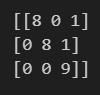
\includegraphics[scale=1]{gambar/cfrbf.jpg}
  % Keterangan gambar yang diinputkan
  \caption{Confusion Matrix SVM RBF Kernel}
  % Label referensi dari gambar yang diinputkan
  \label{fig:evalconfRBF}
\end{figure}

\begin{figure} [H] \centering
  % Nama dari file gambar yang diinputkan
  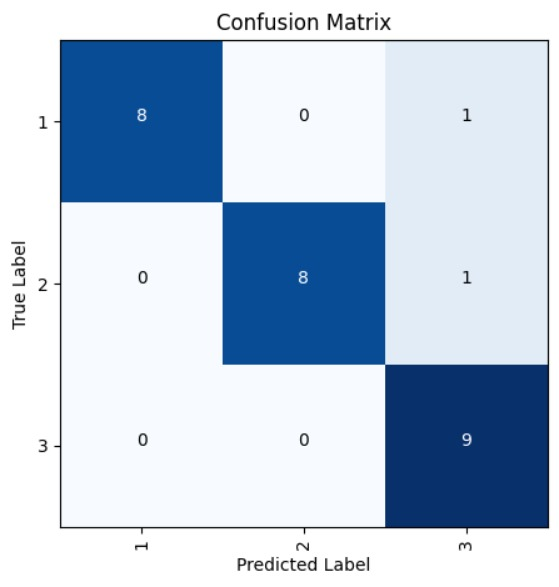
\includegraphics[scale=0.65]{gambar/cfprbf.jpg}
  % Keterangan gambar yang diinputkan
  \caption{visualisasi Confusion Matrix SVM RBF Kernel}
  % Label referensi dari gambar yang diinputkan
  \label{fig:evalconfpRBF}
\end{figure}


\begin{figure} [H] \centering
  % Nama dari file gambar yang diinputkan
  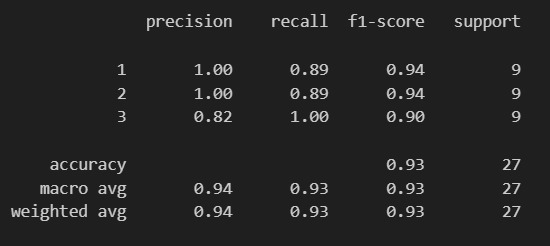
\includegraphics[scale=0.65]{gambar/evalrbf.jpg}
  % Keterangan gambar yang diinputkan
  \caption{Evaluasi SVM RBF Kernel}
  % Label referensi dari gambar yang diinputkan
  \label{fig:evalRBF}
\end{figure}

\subsection{SVM Linear Kernel}
\label{sec:evalLinearKernel}
Pada gambar 4.4 ditampilkan confusion matrix dari hasil evaluasi model SVM dengan kernel Linear. Confusion matrix ini menunjukkan jumlah prediksi benar dan salah yang dibuat oleh model pada data uji. Terlihat bahwa model mampu memprediksi dengan benar 8 sampel kelas 1, 8 sampel kelas 2, dan 9 sampel kelas 3. Namun, terdapat beberapa kesalahan prediksi di mana 1 sampel kelas 1 diprediksi sebagai kelas 3, dan 1 sampel kelas 2 diprediksi sebagai kelas 1.

Visualisasi confusion matrix pada gambar 4.5 memperlihatkan distribusi prediksi model dengan lebih jelas. Warna yang lebih gelap menunjukkan jumlah prediksi yang lebih banyak, yang mengindikasikan bahwa sebagian besar sampel diuji telah diprediksi dengan benar oleh model.

Gambar 4.6 menampilkan laporan klasifikasi yang mencakup metrik-metrik evaluasi seperti precision, recall, f1-score, dan support untuk setiap kelas. Dari tabel ini dapat dilihat bahwa model memiliki precision sebesar 0.89 untuk kelas 1, 0.89 untuk kelas 2, dan 1.00 untuk kelas 3. Recall untuk kelas 1 adalah 0.89, untuk kelas 2 adalah 0.89, dan untuk kelas 3 adalah 1.00. Nilai f1-score menunjukkan keseimbangan antara precision dan recall, dengan nilai tertinggi pada kelas 3 (0.95) dan sedikit lebih rendah pada kelas 1 dan kelas 2 (0.89). Akurasi keseluruhan model adalah 0.89, yang berarti model mampu memprediksi dengan benar 89\% dari total sampel uji. Nilai rata-rata makro (macro avg) dan rata-rata berbobot (weighted avg) untuk precision, recall, dan f1-score juga menunjukkan performa model yang cukup baik.

\begin{figure} [H] \centering
  % Nama dari file gambar yang diinputkan
  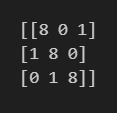
\includegraphics[scale=1]{gambar/cflinear.jpg}
  % Keterangan gambar yang diinputkan
  \caption{Confusion Matrix SVM Linear Kernel}
  % Label referensi dari gambar yang diinputkan
  \label{fig:evalconflinearkernel}
\end{figure}

\begin{figure} [H] \centering
  % Nama dari file gambar yang diinputkan
  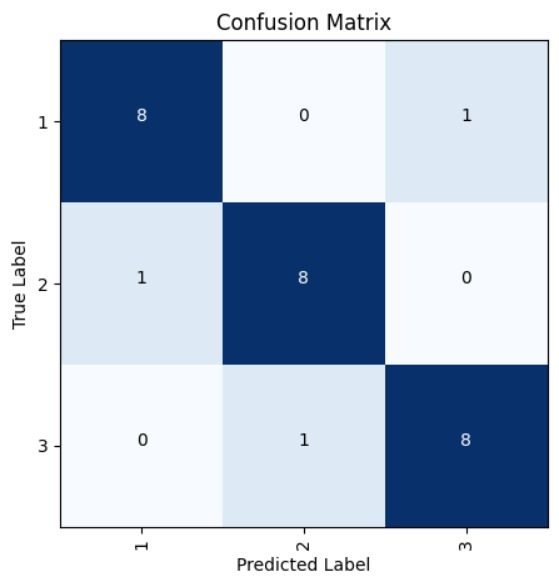
\includegraphics[scale=0.65]{gambar/cfplinear.jpg}
  % Keterangan gambar yang diinputkan
  \caption{Visualisasi Confusion Matrix SVM Linear Kernel}
  % Label referensi dari gambar yang diinputkan
  \label{fig:evalcfplinearkernel}
\end{figure}

\begin{figure} [H] \centering
  % Nama dari file gambar yang diinputkan
  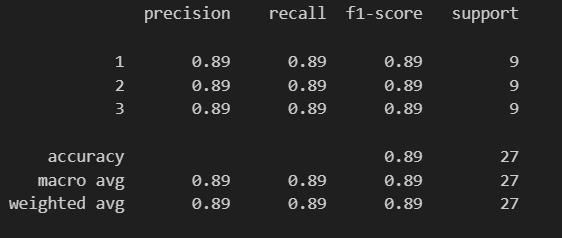
\includegraphics[scale=0.65]{gambar/EvalLinear.jpg}
  % Keterangan gambar yang diinputkan
  \caption{Evaluasi SVM Linear Kernel}
  % Label referensi dari gambar yang diinputkan
  \label{fig:evallinearkernel}
\end{figure}



\subsection{SVM Sigmoid Kernel}
\label{sec:evalSigmoidKernel}

Pada gambar 4.7 ditampilkan confusion matrix dari hasil evaluasi model SVM dengan kernel Sigmoid. Confusion matrix ini menunjukkan jumlah prediksi benar dan salah yang dibuat oleh model pada data uji. Terlihat bahwa model mampu memprediksi dengan benar 8 sampel kelas 1, 8 sampel kelas 2, dan 8 sampel kelas 3. Namun, terdapat beberapa kesalahan prediksi di mana 1 sampel kelas 1 diprediksi sebagai kelas 3, 1 sampel kelas 2 diprediksi sebagai kelas 1, dan 1 sampel kelas 3 diprediksi sebagai kelas 1.

Visualisasi confusion matrix pada gambar 4.8 memperlihatkan distribusi prediksi model dengan lebih jelas. Warna yang lebih gelap menunjukkan jumlah prediksi yang lebih banyak, yang mengindikasikan bahwa sebagian besar sampel diuji telah diprediksi dengan benar oleh model.

Gambar 4.9 menampilkan laporan klasifikasi yang mencakup metrik-metrik evaluasi seperti precision, recall, f1-score, dan support untuk setiap kelas. Dari tabel ini dapat dilihat bahwa model memiliki precision sebesar 0.89 untuk kelas 1, 1.00 untuk kelas 2, dan 0.89 untuk kelas 3. Recall untuk kelas 1 adalah 0.89, untuk kelas 2 adalah 0.89, dan untuk kelas 3 adalah 0.89. Nilai f1-score menunjukkan keseimbangan antara precision dan recall, dengan nilai tertinggi pada kelas 2 (0.94) dan sedikit lebih rendah pada kelas 1 dan kelas 3 (0.89). Akurasi keseluruhan model adalah 0.89, yang berarti model mampu memprediksi dengan benar 89\% dari total sampel uji. Nilai rata-rata makro (macro avg) dan rata-rata berbobot (weighted avg) untuk precision, recall, dan f1-score juga menunjukkan performa model yang cukup konsisten.

Secara keseluruhan, hasil evaluasi ini menunjukkan bahwa model SVM dengan kernel Sigmoid memiliki kemampuan yang baik dalam mengklasifikasikan sampel-sampel pada data uji, dengan beberapa kesalahan prediksi yang terjadi. Meskipun terdapat beberapa kesalahan dalam prediksi antar kelas, model ini masih menunjukkan tingkat akurasi yang tinggi dan dapat diandalkan untuk tugas klasifikasi pada dataset ini.

\begin{figure} [H] \centering
  % Nama dari file gambar yang diinputkan
  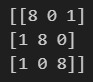
\includegraphics[scale=1]{gambar/cfsigmoid.jpg}
  % Keterangan gambar yang diinputkan
  \caption{Confusion Matrix SVM Sigmoid Kernel}
  % Label referensi dari gambar yang diinputkan
  \label{fig:evalcfsigmoidkernel}
\end{figure}

\begin{figure} [H] \centering
  % Nama dari file gambar yang diinputkan
  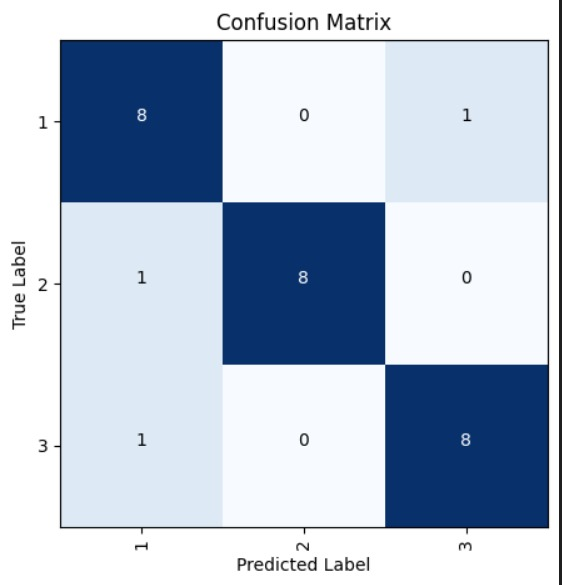
\includegraphics[scale=0.65]{gambar/cfpsigmoid.jpg}
  % Keterangan gambar yang diinputkan
  \caption{Visualisasi Confusion Matrix SVM Sigmoid Kernel}
  % Label referensi dari gambar yang diinputkan
  \label{fig:evalcfpsigmoidkernel}
\end{figure}

\begin{figure} [H] \centering
  % Nama dari file gambar yang diinputkan
  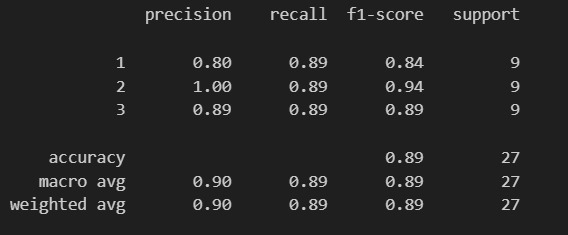
\includegraphics[scale=0.65]{gambar/evalsigmoid.jpg}
  % Keterangan gambar yang diinputkan
  \caption{Evaluasi SVM Sigmoid Kernel}
  % Label referensi dari gambar yang diinputkan
  \label{fig:evalsigmoidkernel}
\end{figure}


\subsection{SVM Polynomial Kernel}
\label{sec:evalPolyKernel}


Pada gambar 4.10 ditampilkan confusion matrix dari hasil evaluasi model SVM dengan kernel Polynomial. Confusion matrix ini menunjukkan jumlah prediksi benar dan salah yang dibuat oleh model pada data uji. Terlihat bahwa model mampu memprediksi dengan benar 9 sampel kelas 1, 8 sampel kelas 2, dan 7 sampel kelas 3. Namun, terdapat beberapa kesalahan prediksi di mana 1 sampel kelas 2 diprediksi sebagai kelas 1, dan 1 sampel kelas 3 diprediksi sebagai kelas 1.

Visualisasi confusion matrix pada gambar 4.11 memperlihatkan distribusi prediksi model dengan lebih jelas. Warna yang lebih gelap menunjukkan jumlah prediksi yang lebih banyak, yang mengindikasikan bahwa sebagian besar sampel diuji telah diprediksi dengan benar oleh model.

Gambar 4.12 menampilkan laporan klasifikasi yang mencakup metrik-metrik evaluasi seperti precision, recall, f1-score, dan support untuk setiap kelas. Dari tabel ini dapat dilihat bahwa model memiliki precision sebesar 0.82 untuk kelas 1, 0.89 untuk kelas 2, dan 1.00 untuk kelas 3. Recall untuk kelas 1 adalah 1.00, untuk kelas 2 adalah 0.89, dan untuk kelas 3 adalah 0.78. Nilai f1-score menunjukkan keseimbangan antara precision dan recall, dengan nilai tertinggi pada kelas 1 (0.90) dan sedikit lebih rendah pada kelas 2 (0.89) dan kelas 3 (0.88). Akurasi keseluruhan model adalah 0.89, yang berarti model mampu memprediksi dengan benar 89\% dari total sampel uji. Nilai rata-rata makro (macro avg) dan rata-rata berbobot (weighted avg) untuk precision, recall, dan f1-score juga menunjukkan performa model yang cukup baik.

\begin{figure} [H] \centering
  % Nama dari file gambar yang diinputkan
  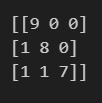
\includegraphics[scale=1]{gambar/cfpoly.jpg}
  % Keterangan gambar yang diinputkan
  \caption{Confusion Matrix SVM Polynomial Kernel}
  % Label referensi dari gambar yang diinputkan
  \label{fig:evalcfpolykernel}
\end{figure}

\begin{figure} [H] \centering
  % Nama dari file gambar yang diinputkan
  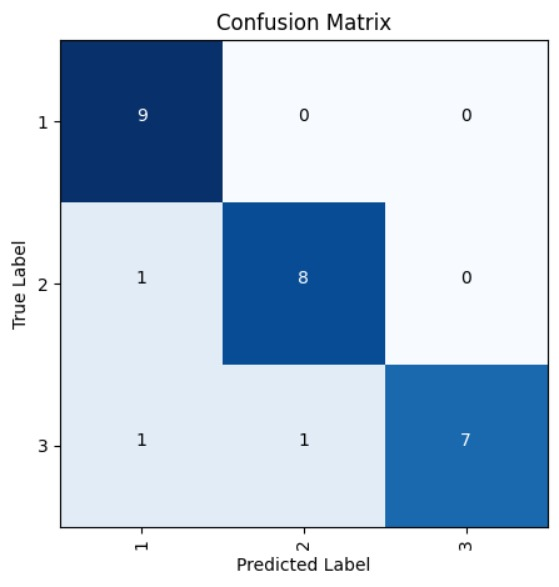
\includegraphics[scale=0.65]{gambar/cfppoly.jpg}
  % Keterangan gambar yang diinputkan
  \caption{Visualisasi Confusion Matrix SVM Polynomial Kernel}
  % Label referensi dari gambar yang diinputkan
  \label{fig:evalcfppolykernel}
\end{figure}

\begin{figure} [H] \centering
  % Nama dari file gambar yang diinputkan
  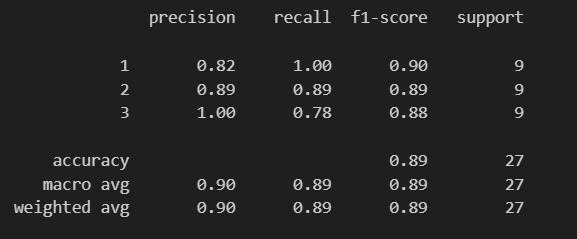
\includegraphics[scale=0.65]{gambar/evalpoly.jpg}
  % Keterangan gambar yang diinputkan
  \caption{Evakuasi SVM Polynomial Kernel}
  % Label referensi dari gambar yang diinputkan
  \label{fig:evalpolykernel}
\end{figure}

\subsection{Multi-Layer Perceptron (\emph{MLP})}
\label{sec:evalSigmoidKernel}

Pada gambar 4.13 ditampilkan confusion matrix dari hasil evaluasi model Multi-Layer Perceptron (MLP) selama proses training. Confusion matrix ini menunjukkan jumlah prediksi benar dan salah yang dibuat oleh model pada data uji. Terlihat bahwa model mampu memprediksi dengan benar 8 sampel kelas 1, 8 sampel kelas 2, dan 8 sampel kelas 3. Namun, terdapat beberapa kesalahan prediksi di mana 1 sampel kelas 1 diprediksi sebagai kelas 3, 1 sampel kelas 2 diprediksi sebagai kelas 1, dan 1 sampel kelas 3 diprediksi sebagai kelas 1.

Visualisasi confusion matrix pada gambar 4.14 memperlihatkan distribusi prediksi model dengan lebih jelas. Warna yang lebih gelap menunjukkan jumlah prediksi yang lebih banyak, yang mengindikasikan bahwa sebagian besar sampel diuji telah diprediksi dengan benar oleh model.

Gambar 4.15 menampilkan laporan klasifikasi yang mencakup metrik-metrik evaluasi seperti precision, recall, f1-score, dan support untuk setiap kelas. Dari tabel ini dapat dilihat bahwa model memiliki precision sebesar 0.80 untuk kelas 1, 1.00 untuk kelas 2, dan 0.89 untuk kelas 3. Recall untuk kelas 1 adalah 0.89, untuk kelas 2 adalah 0.89, dan untuk kelas 3 adalah 0.89. Nilai f1-score menunjukkan keseimbangan antara precision dan recall, dengan nilai tertinggi pada kelas 2 (0.94) dan sedikit lebih rendah pada kelas 1 (0.84) dan kelas 3 (0.89). Akurasi keseluruhan model adalah 0.89, yang berarti model mampu memprediksi dengan benar 89\% dari total sampel uji. Nilai rata-rata makro (macro avg) dan rata-rata berbobot (weighted avg) untuk precision, recall, dan f1-score juga menunjukkan performa model yang cukup konsisten.

Arsitektur model yang digunakan pada training ini adalah MLP dengan dua lapisan tersembunyi yang terdiri dari 5 dan 2 neuron masing-masing. Model dilatih menggunakan fungsi aktivasi ReLU (Rectified Linear Unit) dan solver Adam untuk optimasi. Jumlah iterasi maksimum yang digunakan adalah 100000, yang memastikan bahwa model mencapai konvergensi selama proses training. Akurasi model yang dicapai adalah 0.89, menunjukkan bahwa model ini memiliki kemampuan yang baik dalam mengklasifikasikan sampel-sampel pada data uji.

\begin{figure} [H] \centering
  % Nama dari file gambar yang diinputkan
  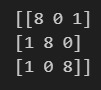
\includegraphics[scale=1]{gambar/cfmlp.jpg}
  % Keterangan gambar yang diinputkan
  \caption{Confusion Matrix MLP training}
  % Label referensi dari gambar yang diinputkan
  \label{fig:evalcfmlp}
\end{figure}

\begin{figure} [H] \centering
  % Nama dari file gambar yang diinputkan
  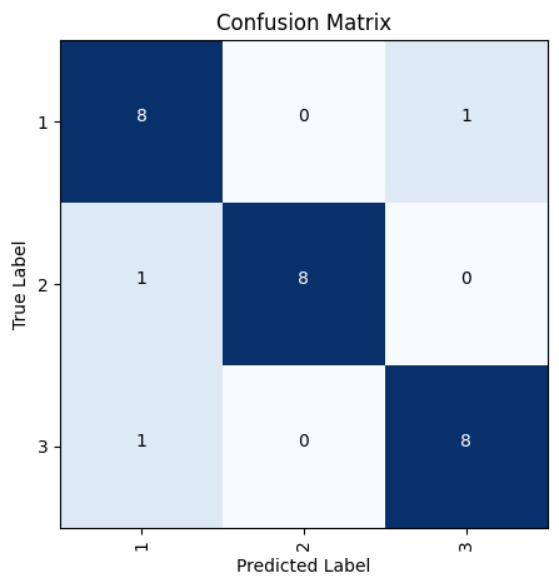
\includegraphics[scale=0.65]{gambar/cfpmlp.jpg}
  % Keterangan gambar yang diinputkan
  \caption{Visualisasi Confusion Matrix MLP training}
  % Label referensi dari gambar yang diinputkan
  \label{fig:evalcfpmlp}
\end{figure}

\begin{figure} [H] \centering
  % Nama dari file gambar yang diinputkan
  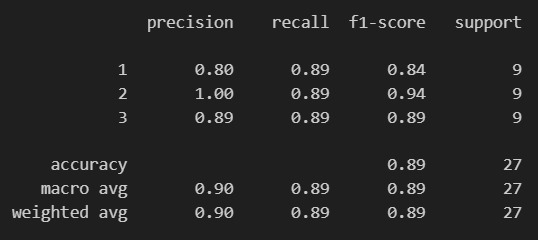
\includegraphics[scale=0.65]{gambar/evalmlp.jpg}
  % Keterangan gambar yang diinputkan
  \caption{Evaluasi Hasil training MLP}
  % Label referensi dari gambar yang diinputkan
  \label{fig:evalmlpl}
\end{figure}

\begin{figure} [H] \centering
  % Nama dari file gambar yang diinputkan
  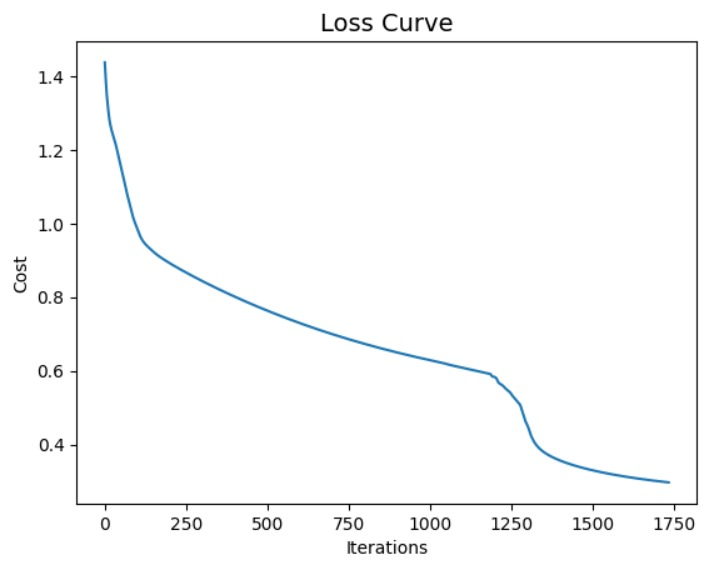
\includegraphics[scale=0.5]{gambar/lossmlp.jpg}
  % Keterangan gambar yang diinputkan
  \caption{Loss training MLP}
  % Label referensi dari gambar yang diinputkan
  \label{fig:lossmlp}
\end{figure}

\section{Hasil Pengujian Model}
\label{sec:skenariopengujian}
\begin{figure} [H] \centering
  % Nama dari file gambar yang diinputkan
  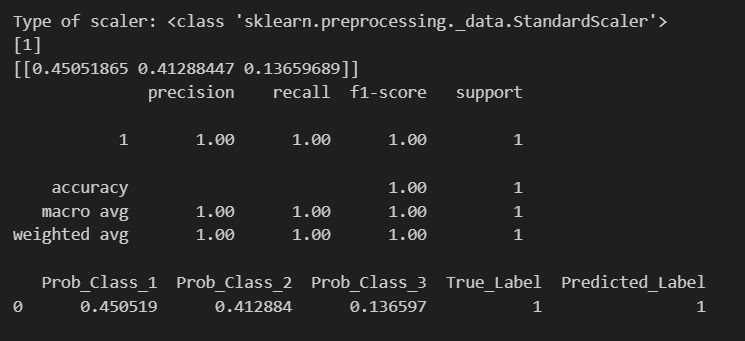
\includegraphics[scale=0.75]{gambar/predik.jpg}
  % Keterangan gambar yang diinputkan
  \caption{Hasil pengujian model}
  % Label referensi dari gambar yang diinputkan
  \label{fig:predikmodel}
\end{figure}


\section{Pembahasan}
\label{sec:skenariopengujian}


% \section{Evaluasi Pengujian}
% \label{sec:analisispengujian}

% Dari pengujian yang \lipsum[1]

% % Contoh pembuatan tabel

% \lipsum[2-4]
